\documentclass{beamer}
\usetheme{metropolis}

\usepackage{tikz}
\usepackage{dirtytalk}
\usepackage{hyperref}
\usepackage{listings}
\usepackage{color}
\definecolor{atomPurple}{RGB}{198,120,221}
\definecolor{atomRed}{RGB}{203,15,64}
\definecolor{atomGreen}{RGB}{0,128,0}
\definecolor{atomGreyLight}{RGB}{171,178,191}
\definecolor{atomGreyDark}{RGB}{92,99,112}
\definecolor{atomBlack}{RGB}{56,58,66}

\lstset{
language=C,
numbers=left,
showstringspaces=false,
tabsize=4,
columns=flexible,
keepspaces=true,
keywordstyle=\color{atomRed},
stringstyle=\color{atomGreen},
commentstyle=\color{atomGreyDark}
}

\newcommand\heading[1]{%
  \par\bigskip
  {\Large\bfseries#1}\par\smallskip}

\title{Like the Clappers - The Story of an Indexer}
\author{Vaughan Kitchen}
\date{November 5, 2019}

\begin{document}

\begin{frame}
\titlepage
\end{frame}

\begin{frame}{At the Beginning}
	\say{
No student has ever written an indexer faster than mine
	}
	\rightline{{\rm --- Andrew Trotman}}

\end{frame}

\begin{frame}{Months of Programming Later}
	\begin{center}
	\begin{tabular}{c c}
		\textbf{engine} & \textbf{time (s)} \\
		\hline
		ATIRE & 8.27 \\
		\textbf{cocomel} & 6.46 \\
		JASSjr & 19.30 \\
		JASSjr-Java & 29.78 \\
		rangahautia & 17.75 \\
	\end{tabular}
	\end{center}
\end{frame}

\begin{frame}{Test Details}
	\begin{itemize}
	\item WSJ collection: a 500mb XML file
	\item Run 3 times. Take the lowest time
	\item Late 2013 Mac - Intel Core i5-4570 @ 3.20GHz - 8GB 1600MHz DDR3
	\end{itemize}
\end{frame}

\begin{frame}{Now}
	\say{
No student has ever written a UTF-8 indexer faster than mine
	}
	\rightline{{\rm --- Andrew Trotman}}

\end{frame}

\begin{frame}{What This Talk Will Be}
	\begin{itemize}
	\item A lot of exploration through my Git history
	\item A little bit of guidelines for writing performant code
	\end{itemize}
\end{frame}

\begin{frame}{How to Make Fast}
	\begin{itemize}
	\item Choose your language
	\item Choose your data structures
	\item Tune everything
	\item The last 20\% is the hardest
	\end{itemize}
\end{frame}

\begin{frame}{Language Choice}
	\begin{itemize}
	\item C
	\item C++
	\item Fortran
	\item Anything else at your peril
	\item (I'm aware of Rust. Prove me it's faster)
	\end{itemize}
\end{frame}

\begin{frame}{Data Structures - Building a Search Engine}
	\begin{itemize}
	\item Bitstring Signature Files \\
	\hspace{23pt}\begin{tikzpicture}
	\foreach \doc in {0, 1, 2, 3, 4, 5, 6, 7}
		\draw (\doc*0.3+0.15+4, 1pt) -- (\doc*0.3+0.15+4, 0) node[anchor=south] {\tiny $\doc$};
	\end{tikzpicture} \\
	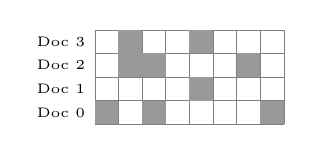
\begin{tikzpicture}
	\foreach \doc in {0, 1, 2, 3}
		\draw (0, \doc*0.3+0.15) -- (0, \doc*0.3+0.15) node[anchor=east] {\tiny Doc \doc};
	\draw[step=0.3cm, gray, very thin] (0, 0) grid (2.4, 1.2);
	% bottom doc
	\fill[black!40!white] (0, 0) rectangle (0.3, 0.3);
	\fill[black!40!white] (0.6, 0) rectangle (0.9, 0.3);
	\fill[black!40!white] (2.1, 0) rectangle (2.4, 0.3);
	% going up
	\fill[black!40!white] (1.2, 0.3) rectangle (1.5, 0.6);
	% almost there
	\fill[black!40!white] (0.3, 0.6) rectangle (0.6, 0.9);
	\fill[black!40!white] (0.6, 0.6) rectangle (0.9, 0.9);
	\fill[black!40!white] (1.8, 0.6) rectangle (2.1, 0.9);
	% top doc
	\fill[black!40!white] (0.3, 0.9) rectangle (0.6, 1.2);
	\fill[black!40!white] (1.2, 0.9) rectangle (1.5, 1.2);
	\end{tikzpicture}
	\item Inverted Index \\
	\begin{tabular}{l c l}
	of & $\rightarrow$ & 1 \\
	Otago & $\rightarrow$ & 1, 2, 3 \\
	University & $\rightarrow$ & 1, 2 \\
	\end{tabular}
	\end{itemize}
\end{frame}

\defverbatim[colored]\searchone{\begin{lstlisting}
std::map<std::string, std::vector<size_t> > postings;
do {
    token = tokenizer_next(tok);
    std::string word(token.value);
    std::vector<size_t> docs;
    postings[word] = docs;
    postings[word].push_back(token.doc_number);
} while (token.type != END);
\end{lstlisting}
}

\begin{frame}{First Attempt}
	\begin{itemize}
	\item Commit: 5d671da
	\item Date: Aug 21, 2018
	\item Msg: Basic slow single word search
	\item Time: 353s
	\item Notes: Trees move slowly
	\end{itemize}
	\searchone


\end{frame}

\begin{frame}{Oh Man Bugs...}
	\begin{itemize}
	\item Commit: 99f5cb6
	\item Date: Aug 31, 2018
	\item Msg: Switch to LIBAVL version of RBT to stop values getting lost
	\item Time: 20.18s
	\item Notes: Hash table with Red-Black Tree. Custom Malloc. Compression
	\item Revert features from here to show the effect on performance
	\end{itemize}
\end{frame}

\begin{frame}{Smaller is Faster?}
	\begin{itemize}
	\item Commit: 88f99ca
	\item Date: Aug 30, 2018
	\item Msg: Compress postings
	\item Time (previous): 20.18s
	\item Time (removed): 26.18s
	\item Notes: 2642, 2646, 2656, 2657 $\rightarrow$ 2642, 4, 10, 1
	\item Notes: Variable byte compression means most values are 8bits
	\end{itemize}
\end{frame}

\defverbatim[colored]\logkmerge{\begin{lstlisting}
for (size_t gap = 1; gap < h->capacity; gap *= 2) {
    for (size_t i = 0; i < h->capacity; i += gap * 2) {
        if (h->store[i] == NULL) {
            h->store[i] = h->store[i+gap];
            continue;
        }
    rbt_kv_merge_left(h->store[i], h->store[i+gap]);
    }
}
\end{lstlisting}
}

\begin{frame}{$n \log(k)$ Beats $O(n^2)$}
	\begin{itemize}
	\item Commit: a069ca1
	\item Date: Aug 29, 2018
	\item Msg: log k merge
	\item Time (previous): 26.18s
	\item Time (removed): 243.83s - beats 353s with map
	\end{itemize}
	\logkmerge
\end{frame}

\begin{frame}{Avoid Syscalls}
	\begin{itemize}
	\item Commit: 5f6377c
	\item Date: Aug 22, 2018
	\item Msg: Custom malloc
	\item Time (previous): 26.18s - before compression, after log k merge
	\item Time (removed): 32.11s
	\item Notes: Take large blocks of memory from malloc and hand it out in chunks - this is a linear allocator
	\end{itemize}
\end{frame}

\begin{frame}{Know Your Data}
	\begin{itemize}
	\item Commit: e2319b8
	\item Date: Sep 3, 2018
	\item Msg: Use plain BST to back hash table. Input guaranteed random and a BST takes less work than an RBT
	\item Time (previous): 20.18s
	\item Time: 13.72s
	\item Notes: Came from talking to Andrew. RBT messes up the branch prediction
	\end{itemize}
\end{frame}

\begin{frame}{Don't Believe Everything a Profiler Says}
	\begin{center}
	\begin{tabular}{| l | r | r |}
	\hline
	\multicolumn{3}{| c |}{\textbf{Profiling information (using gprof)}} \\
	\hline
	\textbf{Function}            &          \textbf{\% of total time}      &    \textbf{time (s)} \\
	\hline
	RBT\_find()          &              47.13\%             &        3.90 \\
	BST\_find()          &               28.70\%            &           1.50 \\
	RBT\_insert()       &              0.48\%               &           0.04 \\
	BST\_insert()       &               0.19\%              &           0.01 \\
	\hline
	\end{tabular}
	\end{center}
\end{frame}

\defverbatim[colored]\termcount{\begin{lstlisting}
struct posting {
	size_t id, diff;
	uint8_t count, *id_store;
	size_t id_capacity, id_length;
	dynamic_array<uint8_t> *counts;
};
\end{lstlisting}
}

\begin{frame}{Good Answers Fast Win Over Right Answers}
	\begin{itemize}
	\item Commit: a6ef328
	\item Date: Apr 27, 2019
	\item Msg: Reduce index size by capping term count
	\item Time (previous): 13.72s
	\item Time: 13.08s
	\item Notes: If a term occurs more than 255 times in a document it has negligible effect. Reducing memory usage however improves performance
	\end{itemize}
	\termcount
\end{frame}

\defverbatim[colored]\makenode{\begin{lstlisting}
struct bst_kv_node *make_node(char *key, void *val) {
    struct bst_kv_node *n = memory_alloc(sizeof(*n));
    n->key = string_s_dup(key);
    n->val = val;
    n->link[0] = n->link[1] = NULL;
    return n;
}
\end{lstlisting}
}

\begin{frame}{Don't Alloc What You Don't Need}
	\begin{itemize}
	\item Commit: f971c6c
	\item Date: May 13, 2019
	\item Msg: Reduce string allocation when parsing
	\item Time (previous): 13.08s
	\item Time: 11.96s
	\item Notes: Adding terms is rare. Looking up terms is common
	\end{itemize}
	\makenode
\end{frame}

\begin{frame}{Know Your Lifecycle}
	\begin{itemize}
	\item Commit: 87d9ef7
	\item Date: May 14, 2019
	\item Msg: Use custom allocator in more places as it's generally faster
	\item Time (previous): 11.96s
	\item Time: 10.63s
	\item Notes: Overload the new method in C++ so that class instantiation goes through the linear allocator
	\end{itemize}
\end{frame}

\defverbatim[colored]\hashdiff{\begin{lstlisting}
-    unsigned int hash = htable_word_to_int(key) % h->capacity;
+    unsigned int hash = htable_word_to_int(key) & 0x7FFF;
\end{lstlisting}
}

\begin{frame}{Go Level When Available}
	\begin{itemize}
	\item Commit: dee147d
	\item Date: May 15, 2019
	\item Msg: Slight performance gain in hash function. Increased robustness for NULLs
	\item Time (previous): 10.63s
	\item Time: 9.82s
	\item Notes: Modulo is slow - it requires repeat division
	\end{itemize}
	\hashdiff
\end{frame}

\begin{frame}{Rookie}
	\begin{itemize}
	\item Commit: 30787ec
	\item Date: May 27, 2019
	\item Msg: Write the hash table as the index without conversion
	\item Time (previous): 9.82s
	\item Time: 9.02s
	\item Notes: Why convert the hash table to an ordered list when it can be searched directly? Rookie
	\end{itemize}
\end{frame}

\begin{frame}{Keep Related Data Together}
	\begin{itemize}
	\item Commit: aae4014
	\item Date: Jun 8, 2019
	\item Msg: Refactor to be more truly C++
	\item Time (previous): 9.02s
	\item Time: 8.01s
	\item Notes: Low hanging fruit of value vs reference types gobbled up. Closer storage of related values
	\end{itemize}
\end{frame}

\begin{frame}{Inline Everything}
	\begin{itemize}
	\item Commits: f33d200, b0b9fe
	\item Date: Jun 10, 2019
	\item Msg: Faster implementations of ctype functions
	\item Msg: Inline strcmp
	\item Time (previous): 8.01s
	\item Time: 6.43s
	\item Notes: Function calls are expensive
	\item Notes: Actually inlining everything would be slow due to throwing out the instruction cache
	\end{itemize}
\end{frame}

\begin{frame}{Things That Are Slow}
	\begin{itemize}
	\item Function calls
	\item Branch misprediction
	\item Memory access
	\item System calls
	\item Bad algorithms
	\end{itemize}
\end{frame}

\begin{frame}{Questions?}
	\heading{Find me}
	\begin{itemize}
	\item http://vaughan.kitchen
	\item https://github.com/vkitchen/cocomel
	\end{itemize}
	\heading{Questions?}
\end{frame}

\end{document}
